\chapter{Literature Review}
\label{literature}
This chapter will present the background information and approaches for deep learning (Section 2.1) and discuss the most prevalent techniques and evaluation methods in machine translation (Section 2.2). It will then investigate data augmentation in low-resource machine translation (Section 2.3) and low-resource machine translation (Section 2.4). Finally, the findings will be concluded in the literature review conclusions (Section 2.5).


\clearpage
\section{Deep Learning}
\label{section:deep_learning}

% What is deep learning?
Deep learning is a subset of machine learning inspired by the human brain that uses artificial neural networks with many hidden layers to extract features from inputs while training with large amounts of data.
Deep learning neural networks such as a \acrfull{CNN} expand upon the concept of feedforward neural networks like the perceptron. A single-layer perceptron is the most basic form of neural network that is used for binary classification, with a single layer of output nodes that are connected directly to weighted inputs through an activation function. A multi-layer perceptron expands the single-layer perceptron with the addition of hidden layers, where all nodes in one layer are connected to all the nodes in the next layer, as shown in Figure \ref{fig:perceptron_multi}. The additional layers allow the perceptron to solve nonlinear classification problems (\cite{driss_comparison_2017}).

\begin{figure}[ht!]
\centering
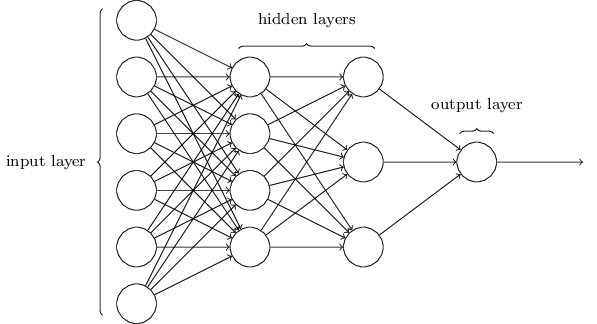
\includegraphics[width=0.65\textwidth]{media/literature/machine_learning/ml_perceptron_multi.png}
\caption[Multi-layer perceptron]{Multi-Layer Perceptron (\cite{michael_perceptron_2019})}
\label{fig:perceptron_multi}
\end{figure}

Extracting simple features from the lower levels of representation helps to identify the abstract features present in the higher representation levels that lead to the output classification of data (\cite{bengio_deep_2011}).
%
The intricacies of a data structure are identified using backpropagation to determine how the neural network should update the weights that are responsible for calculating the representation in each layer, based on the representation of the previous layer. (\cite{lecun_deep_2015}). The proceeding chapters explore the literature surrounding deep learning neural networks, specifically the \acrfull{CNN}, \acrfull{RNN}, and \acrfull{GRU}.

\subsection{Convolutional Neural Networks}

A \acrfull{CNN} is an artificial neural network similar to the multi-layer perceptron with additional hidden convolutional layers. \acrshort{CNN}s are very good at detecting patterns from data which makes them ideal for image classification, object recognition, and more recently \acrfull{NLP} (\cite{young_cnns_recent_2018}).

Research by \cite{lecun_backprop_cnn_1989} was the first to demonstrate how the backpropagation algorithm proposed by \cite{rumelhart_learning_1986} could be integrated into a convolutional neural network.
Using the \acrshort{CNN}, they successfully performed character recognition and classification on images of handwritten digits from data provided by the U.S Postal Service.

The \acrshort{CNN} architecture is shown in Figure \ref{fig:cnn_1} using an example of image classification.

\begin{figure}[ht!]
\centering
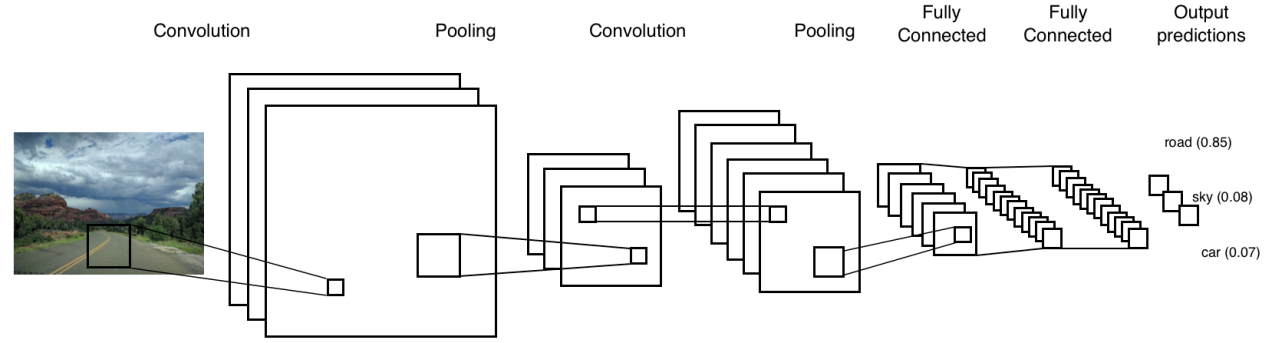
\includegraphics[width=1\textwidth]{media/literature/machine_learning/ml_cnn_1.png}
\caption[Convolutional neural network architecture]{Convolutional Neural Network architecture (\cite{lopez_deep_2017})}
\label{fig:cnn_1}
\end{figure}

A convolutional layer typically involves three different actions (\cite{goodfellow_deep_learning_2016}):
\begin{itemize}
    \item Run multiple convolutions in parallel, producing a set of linear activations
    \item Use a nonlinear activation function on each linear activation
    \item Use a pooling function to downsample the layer output
\end{itemize}


% Convolutional layers + filters
A convolution is a mathematical operation that generates an activation map (matrix) using inputs such as an image matrix and a filter, outputting high values if the convolution feature is present in that location. For image classification, a filter represents a small matrix with a preset number of columns and rows.
A convolutional layer has a specified number of filters that are used to detect different patterns. These filters are initialised with random numbers and adjusted using backpropagation to learn the weights automatically.
When a convolutional layer receives an input, the filter convolves over each $n$ x $n$ block of pixels in the image and the value of each cell becomes the dot product of the block of pixels and the filter. The resultant matrix is used as input to the next layer.

In early convolutional layers, filters may only detect very simple features such as edges and shapes but as the layers get deeper in the neural network, filters can identify more complicated objects such as facial features or types of animals. These high-level features are what the classifier uses for weighting the output predictions.
\acrshort{NLP} tasks consist of text input sentences rather than images so rows within a matrix are word embedding vectors that are generated using models such as word2vec (\cite{mikolov_word2vec_2013}). 
As each row in the matrix represents an entire word, filters span the full width of the row to match the width of the matrix input, with a height of between $2$ - $5$ words (\cite{lopez_deep_2017}).

% Activation function
The activation function of a neural network transforms the weighted input of a neuron into the activation of the output, determining whether a neuron fires or not. Unlike the sigmoid and hyperbolic tangent activation functions that suffer from the vanishing gradient problem, \acrfull{RELU} converges quickly and overcomes the vanishing gradient problem, making it the recommended activation function for modern \acrshort{CNN}s (\cite{nair_rectified_2010}). 
Leaky ReLU is a variation of \acrshort{RELU} that applies a small negative gradient when $x < 0$ to prevent the dying \acrshort{RELU} problem.

% Pooling layer
Feature maps (the output activations for a given filter) are sensitive to the position of a feature in an image. Pooling layers address this issue by reducing the resolution of the feature maps to introduce translation invariance (\cite{scherer_evaluation_2010}). The downsampled feature maps can be thought of as a summary of the nearby outputs present in small $n$ x $n$ patches (the pooling window) of the feature map. The most common methods of pooling are max pooling and average pooling. However, \cite{scherer_evaluation_2010} found that the max pooling operation significantly outperforms subsampling operations.

% Fully connected layers
The fully connected layers take outputs from the convolution and flatten them into a single vector. Using the Softmax activation function, the values of the vector in the final layer represent the probabilities of features matching the labels used for classification. Every neuron has full connections to all of the activations from the previous layer, and activations are computed using matrix multiplication and a bias offset (\cite{stanford_cs231n_2019}).

\begin{figure}[ht!]
\centering
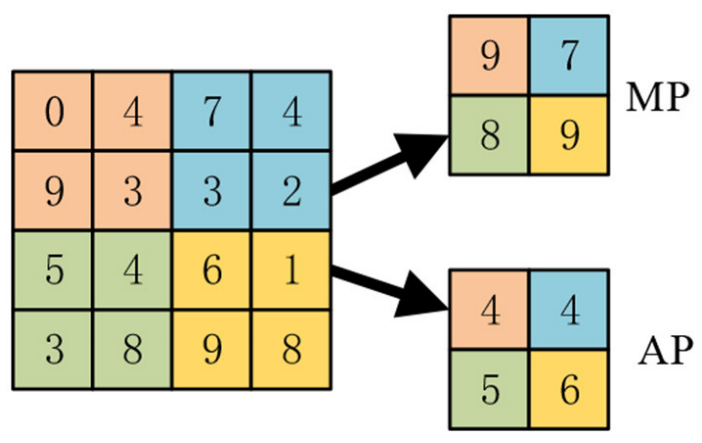
\includegraphics[width=0.30\textwidth]{media/literature/machine_learning/ml_pooling.png}
\caption[CNN max pooling and average pooling ]{\acrshort{CNN} Max Pooling (MP) and Average Pooling (AP) (\cite{wang_pooling_2018})}
\label{fig:cnn_pooling}
\end{figure}

%These pooling methods are visualised in Figure \ref{fig:cnn_pooling}:
As demonstrated in Figure \ref{fig:cnn_pooling}, max pooling and average pooling are carried out by:

\begin{itemize}
    \item Max Pooling: Select the maximum value within the pooling window
    \item Average Pooling: Select the average value within the pooling window
\end{itemize}

% Dropout
Dropout is a technique that helps address the problem of overfitting for \acrshort{CNN}s that have many parameters. During training, a random set of neurons and their subsequent connections in the network are dropped (ignored) with probability $p$ (\cite{srivastava_dropout_2014}). This can be seen in Figure \ref{fig:cnn_dropout}. In the original research by \cite{hinton_dropout_2012}, dropout was only applied to the fully connected layers of a \acrshort{CNN}. However, \cite{lai_dropout_2017} has since found that regularisation increased when dropout is also used after the activation function of every convolutional layer in the network at a lower probability ($p = 0.1$).

\begin{figure}[ht!]
\centering
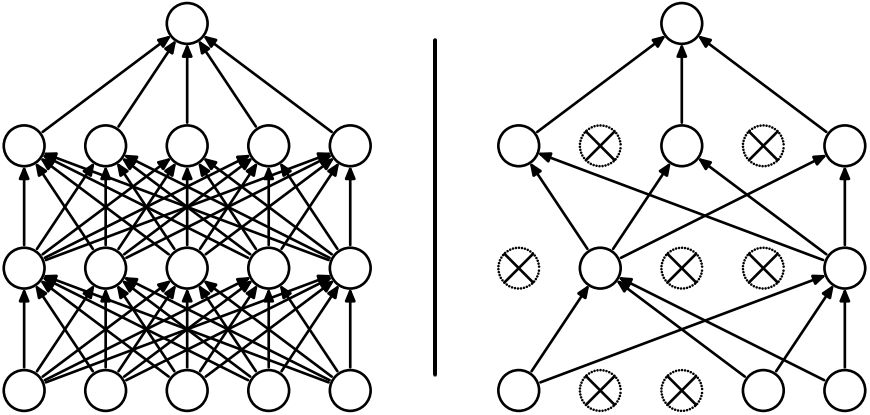
\includegraphics[width=0.55\textwidth]{media/literature/machine_learning/ml_dropout3.png}
\caption[Dropout neural network model]{Dropout neural network model. Left side: Standard \acrshort{NN} with 2 hidden layers. Right side: Standard \acrshort{NN} with 2 hidden layers, after applying dropout (\cite{srivastava_dropout_2014})}
\label{fig:cnn_dropout}
\end{figure}

\subsection{Recurrent Neural Networks}

% Introduction
Traditional neural networks struggle to retain previous information as they only map input vectors to output vectors (\cite{graves_supervised_2012}). A \acrfull{RNN} is a type of neural network that performs the same function at every time step in a sequence, using the output of the previous step as the input to the current step.
Similar to the objectives of traditional neural networks such as a \acrshort{CNN}, an \acrshort{RNN} aims to reduce the loss value between input and output pair predictions using backpropagation to learn the network weights. 
\acrshort{RNN}s are capable of mapping the entire history of previous inputs to each output, using internal hidden states to maintain a representation of the information that has been calculated previously and influence the network output.
% What are they good at?
This is particularly useful for \acrshort{NLP}, where the prediction of a word often depends on the context of what has been observed in the sentence so far. Short term memory also improves the handling of invariance for tasks such as image classification (\cite{mikolov_recurrent_slides_2010}), where the position, orientation, and size of an object may differ but the correct object is still identified. 

The 'simple recurrent neural network' was first proposed by \cite{elman_original_rnn_1990} and consists of an input layer, a recurrent hidden layer, and an output layer. The recurrent hidden layer is essentially multiple copies of the same neural network that are connected sequentially and pass information forwards. The network can be 'unrolled' in a diagram to visualise the sequence, as shown in Figure \ref{fig:rnn_unrolled}.

\begin{figure}[ht!]
\centering
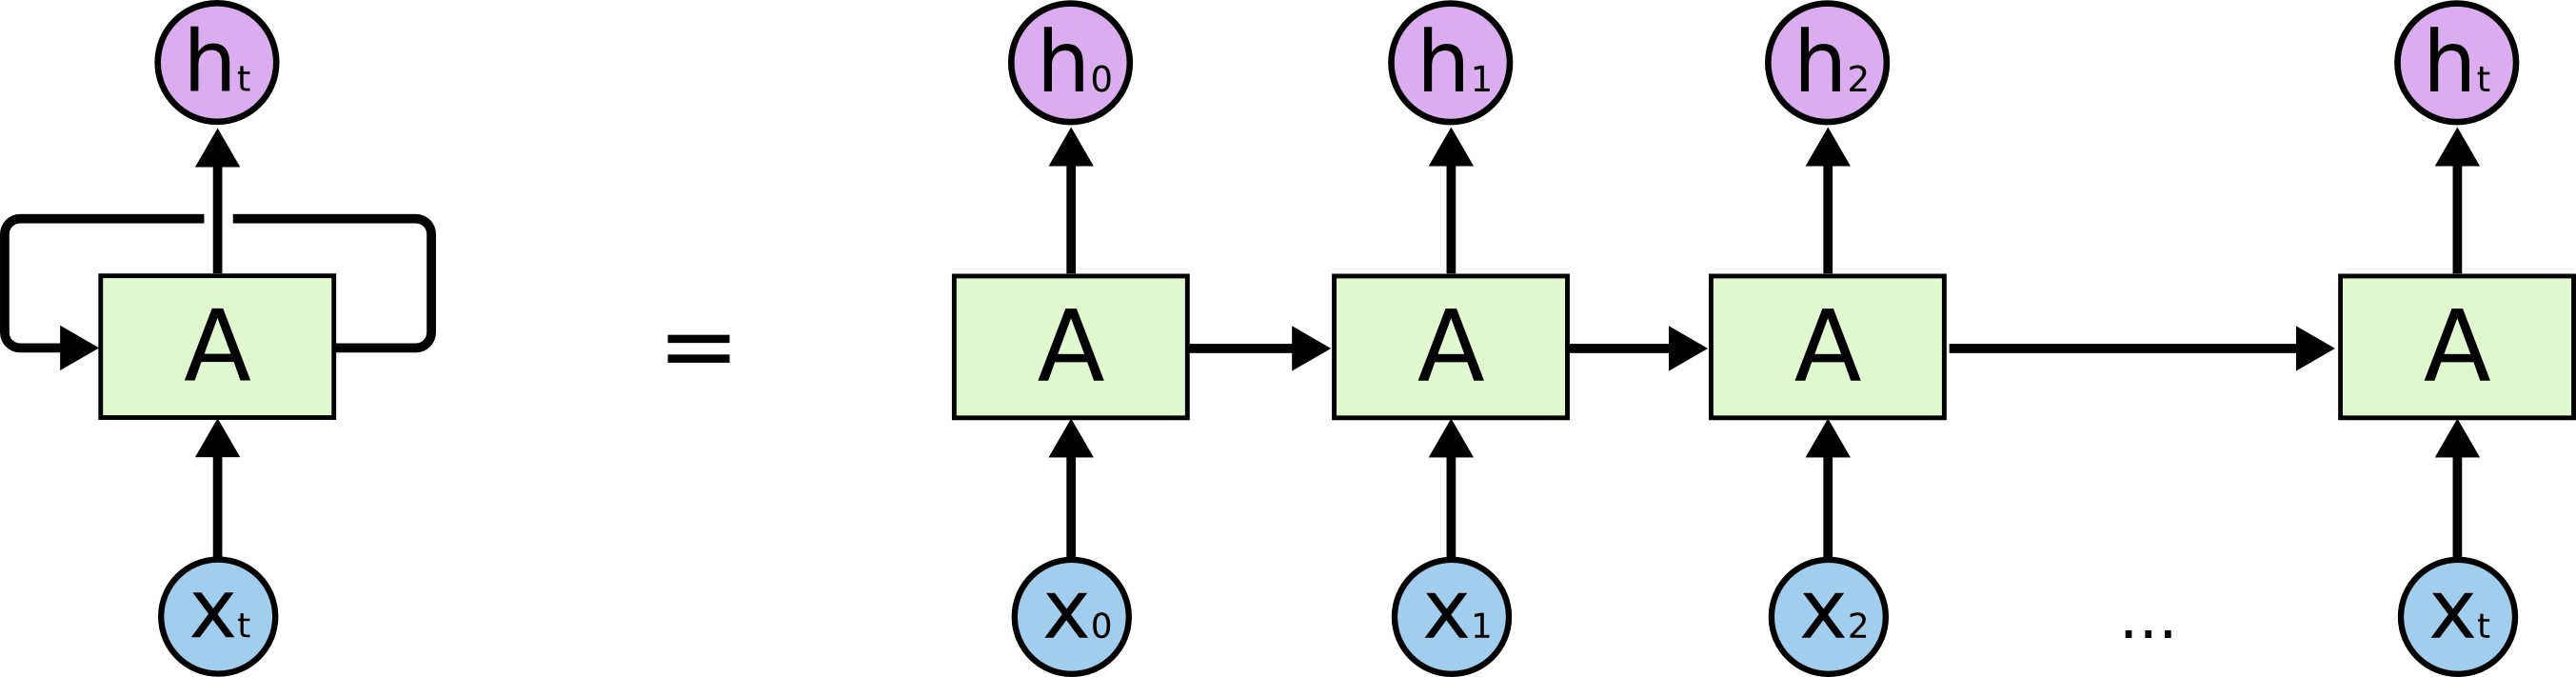
\includegraphics[width=0.9\textwidth]{media/literature/machine_learning/ml_rnn_unrolled.png}
\caption[Unrolled Recurrent Neural Network]{Left side: A vanilla \acrlong{RNN}. Right side: An unrolled vanilla \acrlong{RNN} (\cite{colah_lstm_2019})}
\label{fig:rnn_unrolled}
\end{figure}

To process a sequence of vectors and calculate a new state, a recurrence formula is applied at each time step using a function of the previous state and the current input vector. Regardless of the input or output sequence length, the same function is used at each time step. This is shown below, where $h_t$ is the new state, $f_w$ is a function with parameters W (weights), $h_{t-1}$ is the previous state, and $x_t$ is the input vector at a given time step: 

\begin{equation}
    h_{t} = f_{w} \left ( h_{t-1},x_{t} \right )
\end{equation}

The \acrshort{RNN} receives an input vector every single time step and modifies the internal state. The weights inside the \acrshort{RNN} are used to determine the behaviour of how a state evolves when it receives an input. 
% =========================== Weights are updated using back propagation =========================== 
In a conventional neural network, information travels forwards through the input and output of neurons in the network. The loss value is calculated and then the weights are updated using backpropagation.
In an \acrshort{RNN}, the information output from previous time steps are used as input for future time steps and the loss value is calculated at each time step. In order to minimise the loss value, once the final loss function in the \acrshort{RNN} has been calculated, error signals need to be back-propagated using \acrfull{BPTT} through the entire network to update the weights of every neuron (\cite{salehinejad_recent_rnn_2018}).
% =========================== Then talk about vanishing and exploding gradient problems =========================== 
As outlined by \cite{bengio_learning_1994}, the further back an error signal is back-propagated, the harder it becomes for the network to update the weights. This is known as the vanishing gradient problem, where the gradient reduces such that the weights are essentially prevented from being updated, halting the training progress.
% =========================== Then talk about LSTM =========================== 

\subsubsection{\acrlong{LSTM}}

\acrfull{LSTM} is an \acrshort{RNN} architecture proposed initially by \cite{hochreiter_long_1997} that was designed to help overcome the vanishing gradient problem present during backpropagation. They are significantly better than simple \acrshort{RNN}s at capturing long term dependencies because they use a gradient-based algorithm that enforces a consistent internal state error flow. This ensures that gradients will not become insignificant and halt the learning process.

In the diagram shown in Figure \ref{fig:rnn_lstm}, an entire vector is carried through each line from the output of one node to the input of other nodes. The vectors go through three sigmoid ($\sigma$) gates and one tanh gate (learned neural network layers) to decide what inputs pass through the network and what gets blocked. The symbol in a pink circle denotes the pointwise operation applied to the vectors (addition or multiplication).

\begin{figure}[ht!]
\centering
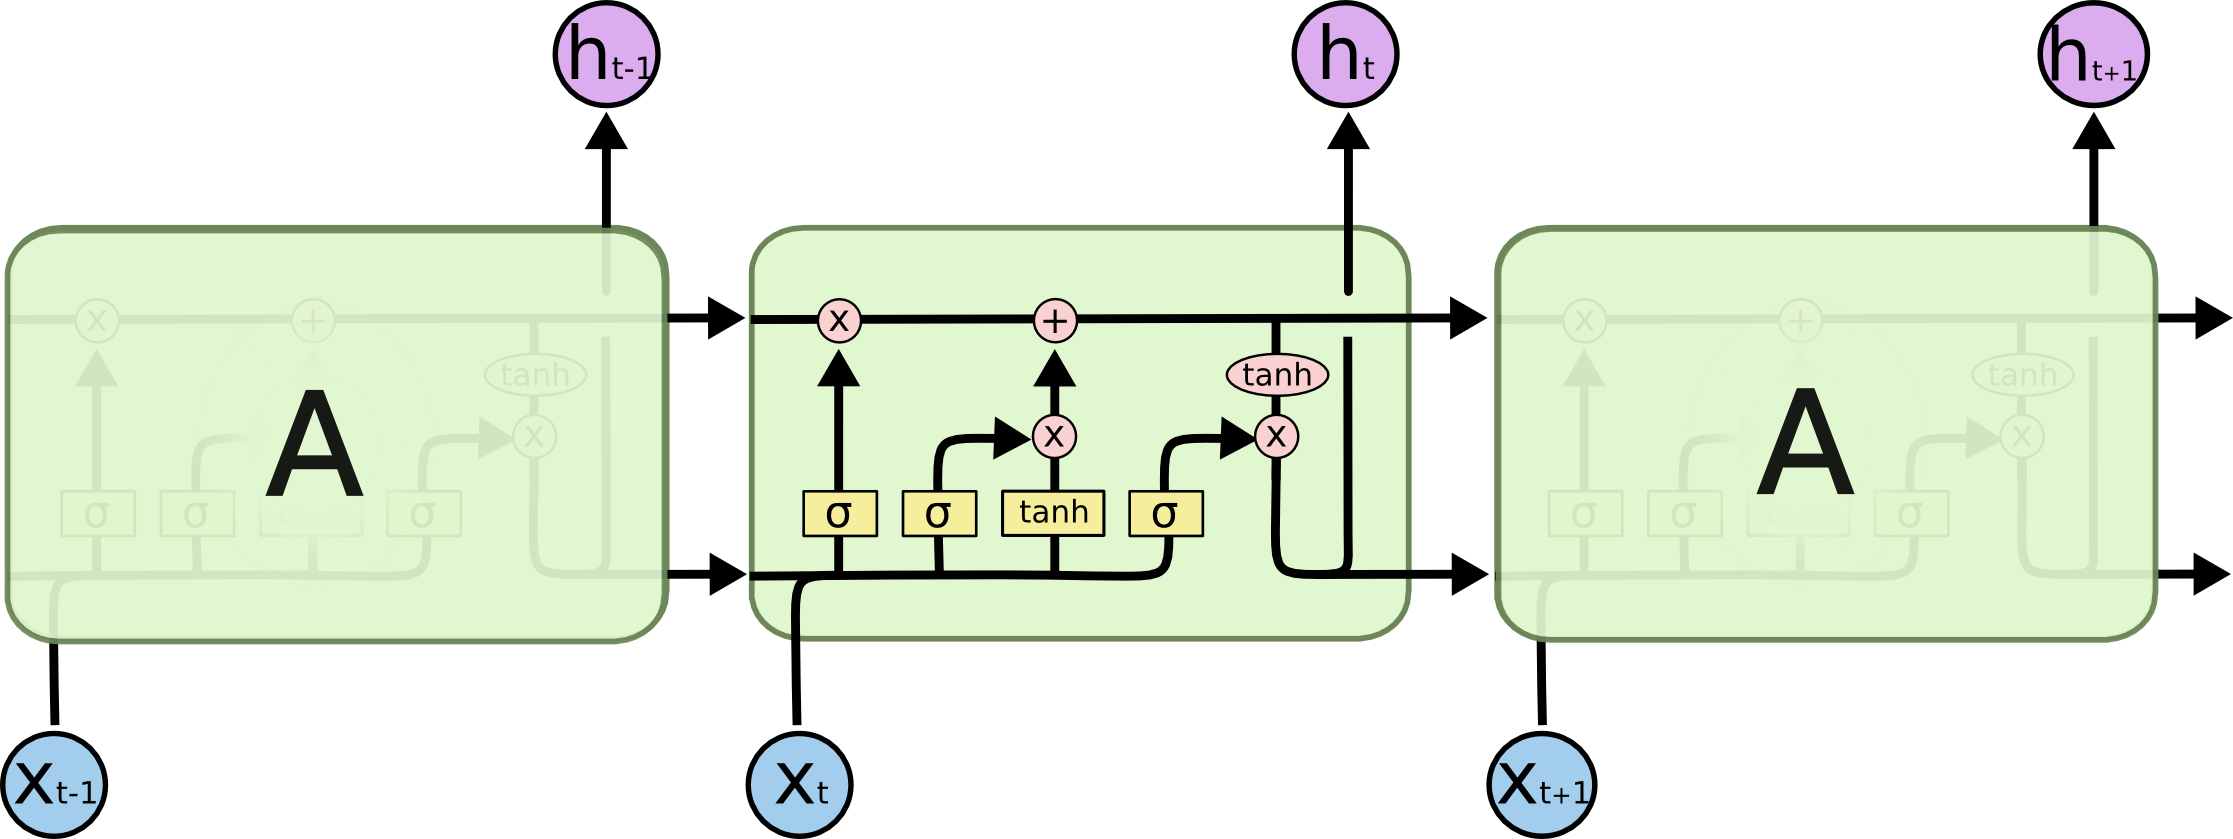
\includegraphics[width=0.89\textwidth]{media/literature/machine_learning/ml_rnn_lstm.png}
\caption[Long Short Term Memory]{\acrfull{LSTM} diagram (\cite{colah_lstm_2019})}
\label{fig:rnn_lstm}
\end{figure}

Predictions are based on the vectors that pass through the gates and a copy is kept for the next time step, meaning future predictions can be informed by memories that haven't forgotten. Referring back to previous time steps allows \acrshort{LSTM}s to better represent language-specific grammar structures and transfer the meaning of sequences to other languages.


One of the issues of using \acrshort{LSTM}s comes from the bandwidth and memory resource constraints that are encountered in the architecture as a result of the high number of tensor operations required. A simpler architecture may be more computationally efficient at the risk of being less accurate for specific deep learning tasks.

% =============== CNN vs LSTM for sequence to sequence ===============

An encoder is a network that maps an input to a feature vector and a decoder is a network that transforms the encoder output into a sequence in the target language. Typically, sequence to sequence problems are solved by stacking both the encoder and decoder with layers of an RNN using \acrshort{LSTM} (\cite{luong_effective_2015}). However, \cite{gehring_convolutional_2017} proposes the first fully connected \acrshort{CNN} for sequence to sequence learning that outperforms high performance \acrshort{LSTM} translation models by up to $1.9$ \acrshort{BLEU}. This approach discovers more compositional structure than \acrshort{RNN}s due to the hierarchical representations of sequences.

\subsubsection{\acrlong{GRU}}

% =============== GRU ===============

\acrfull{GRU} is an architecture proposed by \cite{cho_properties_2014} that consists of an update gate, reset gate, and hidden state. Similar to an \acrshort{LSTM}, a \acrshort{GRU} aims to help overcome the issue of short term memory in \acrshort{RNN}s.
The internal cell state in an \acrshort{LSTM} is not present in a \acrshort{GRU}. Instead, the information is represented in the hidden state vector which is passed onto subsequent \acrshort{GRU}s.
The update gate combines the input and forget gates and is used to determine what information should be learned and discarding the rest, whereas the reset gate decides which information to remove from memory (\cite{gao_gru_2016}).
A diagram of the described architecture can be visualised in more detail in Figure \ref{fig:rnn_gru}.
\begin{figure}[ht!]
\centering
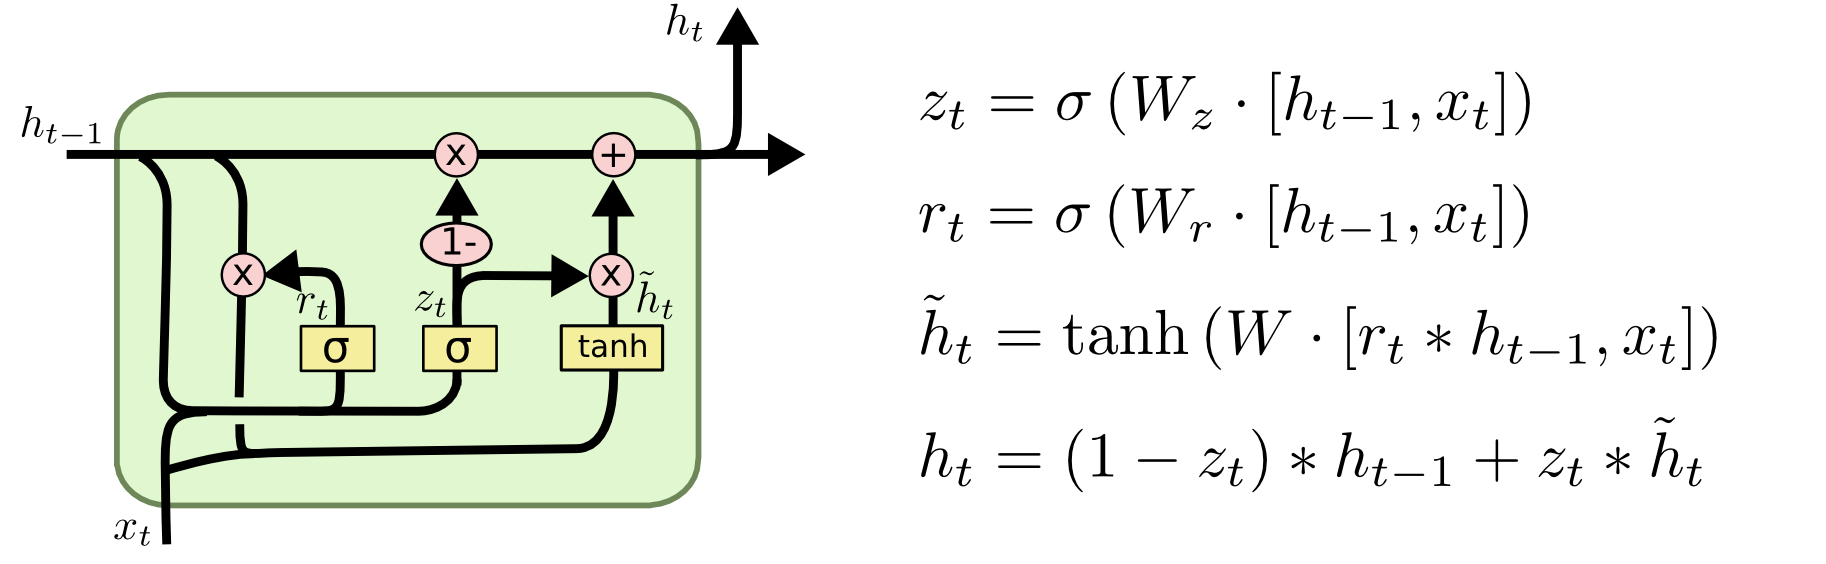
\includegraphics[width=0.89\textwidth]{media/literature/machine_learning/ml_rnn_gru.png}
\caption[Gated Recurrent Unit]{\acrfull{GRU} diagram (\cite{colah_lstm_2019})}
\label{fig:rnn_gru}
\end{figure}

As a result of these differences, \acrshort{GRU}s include fewer tensor operations which can lead to efficient computation and therefore a reduction in training time (\cite{chung_gru_2014}).
The performance of \acrshort{GRU} models favours short sentences without unknown words, degrading significantly as the length of the sentence and unknown word count increases (\cite{cho_properties_2014}).

\section{Machine Translation}
\label{Machine Translation}

This section will introduce machine translation in a review of two of the most prevalent techniques and a review of the literature surrounding metrics for automatic translation evaluations. Subsequent sections will focus on low-resource approaches to \acrshort{NMT} concerning data augmentation and model architectures.

\subsection{Techniques}


\acrfull{SMT} is a statistical approach for machine translation first presented by \cite{brown_statistical_1990}. 
\acrshort{SMT} assumes that all sentences in a source language have the possibility of being the correct translation of a sentence in a target language. 
In other words, find the source sentence $S$ that the translator used to produce the target sentence $T$ by selecting the pair with the highest probability $Pr ( T | S )$.
This is done using a language model, translation model, and decoder as shown in Figure \ref{fig:smt_diagram}.

\begin{figure}[ht!]
\centering
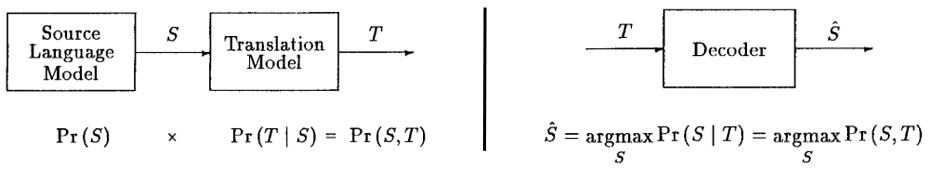
\includegraphics[width=1\textwidth]{media/literature/machine_translation/smt_3.png}
\caption[\acrshort{SMT} probability distribution and decoder]{Left side: \acrshort{SMT} probability distribution for source ($S$) and target ($T$) sentence pairs. Right side: \acrshort{SMT} decoder selecting the highest probability sentence pair (\cite{brown_statistical_1990})}
\label{fig:smt_diagram}
\end{figure}

The language model provides an estimation of how probable a given source sentence is based on the probability distribution of word sequences. This model is associated with the fluency of the translation as it is trained using target language monolingual data, providing the guidelines for well-written translation output. N-grams are all of the combinations of $n$ contiguous words that can be found in a source text. Using a large training corpus, the n-gram probability of every word is determined from the words immediately proceeding it. One drawback to this approach is that the unrecognised increased probability for words that are dependant on each other but are further apart.

The translation model is an estimation of the source and target language vocabulary correspondence. It is associated with the quality of the translations, as it is responsible for predicting the translations of words and short sequences of words, mapping the source language to the target language. Model parameters are estimated by training probabilistic models on large quantities of parallel training data, derived from the following sets of probabilities as proposed by \cite{brown_statistical_1990}:
\begin{itemize}
    \item Fertility probabilities:  $Pr(n|s)$ - the probability that a source word $s$ generates $n$ target words in a given source-target sentence alignment
    
    \item Lexical probabilities: $Pr(s|t)$ - the probability that a source word $s$ translates into a target word $t$, for each element in the source and target language vocabularies
    
    \item Distortion probabilities: $Pr(i|j, l)$ - the probability of the position of a target word $i$, based on the position of the source word $j$, and the length of the target sentence $l$
\end{itemize}

%Explain the decoder
During the runtime of \acrshort{SMT} systems, the decoder uses the translation and language models to find the best translation from the source input to the target language output. 
The decoder starts with an empty hypothesis for the translation. The hypothesis is expanded incrementally by partial hypotheses using the translation and language models. As there is an exponential number of hypotheses concerning the length of the source sentence, search optimisation techniques are required to find the most likely translation. A beam search is an optimised breadth-first search algorithm that searches the most promising nodes, storing and expanding only a limited number of states. In this scenario, it can be used as a decoding technique to confine the search space to a limited quantity of low-cost hypotheses by comparing hypotheses with equal length translation output and removing those with a high cost and estimated future cost (\cite{koehn_pharaoh_2004}).

\subsubsection{Neural Machine Translation}

\acrfull{NMT} is a modern approach to machine translation that uses neural networks to generate statistical models capable of translating sentences from a source language into sentences in the target language.
These models are trained using sequence to sequence learning, where it is possible to map a variable-length input sequence into a variable-length output sequence. %, something that was not possible with conventional \acrshort{DNN}s.
Early research of sequence to sequence neural network models derive from \cite{sutskever_sequence_2014}. They proposed a sequence to sequence solution using the \acrshort{LSTM} architecture that can be simplified into two distinct stages, commonly referred to as an encoder-decoder model:
\begin{itemize}
    \item Encode the input sequence using an \acrshort{LSTM} to create a fixed-length vector
    \item Decode the output sequence from the fixed-length vector using another \acrshort{LSTM}
\end{itemize}

The \acrshort{LSTM} sequence to sequence implementation by \cite{sutskever_sequence_2014} achieved a \acrshort{BLEU} score of $34.8$ on an English to French data set, outperforming a baseline phrased-based \acrshort{SMT} system by $1.5$ \acrshort{BLEU} with the same training corpus.
A generalisation of the encoder-decoder architecture can be visualised in Figure \ref{fig:encoder_decoder}.
\begin{figure}[ht!]
\centering
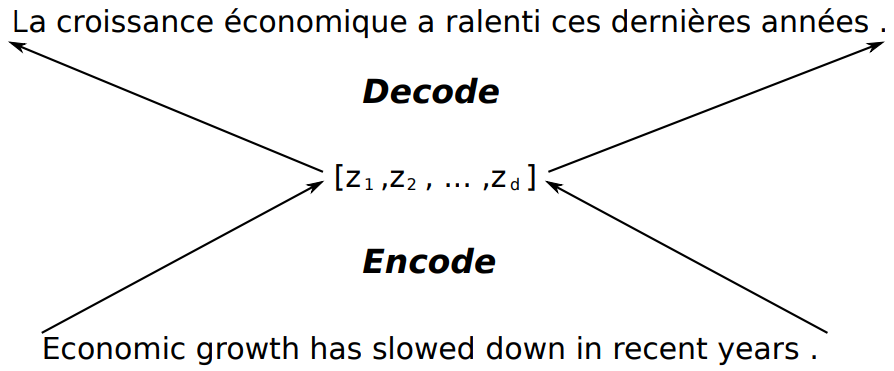
\includegraphics[width=0.64\textwidth]{media/literature/machine_translation/mt_encoder-decoder.png}
\caption[Encoder-decoder architecture]{Encoder-decoder architecture (\cite{cho_properties_2014})}
\label{fig:encoder_decoder}
\end{figure}


% Talk about the encoder-decoder framework
When analysing the properties of \acrshort{NMT} encoder-decoder approaches, \cite{cho_properties_2014} discovered that despite achieving good translation performance on short sentences, when the length of a sentence increases, \acrshort{NMT} translation performance significantly reduces. This is a result of using fixed-length vectors, as longer sentences will struggle to fit within a fixed-length vector without losing certain information, structure, and meaning.

%looks to overcome issues outlined by Cho
It is possible to reduce the likelihood of poor translation quality for long sentences in an encoder-decoder framework by aligning a sequence of vectors with the positions that have the highest concentration of relevant information (\cite{bahdanau_neural_2016}). 
Instead of encoding the entire sentence into one fixed-length vector, each sentence is encoded into a series of vectors. A subset of these vectors is automatically selected during decoding based on previous words and the positions of the relevant information, determining the prediction of the output sequence. This is known as an attention mechanism, due to the ability of the decoder to select which sections of the source sentence to pay attention to during each part of the output sequence. Results of encoder-decoder attention model show significant improvement over conventional \acrshort{NMT} encoder-decoder models, particularly for long sentences (\cite{luong_effective_2015}). Therefore, the implementation of the translation models used for the experimentation of different transfer learning methods in Chapter 3 will include an attention layer.

\subsection{Evaluation}

Although likely to provide a more accurate evaluation of translation quality, hiring professional human translators is costly and time-consuming, making it incompatible with the high output rate of machine translation during training.
Therefore, automatic evaluation plays a key role in the machine translation process, where it is important that translation models can be evaluated quickly and accurately to speed up the training process.

\acrfull{BLEU} is an automatic machine translation algorithm that is widely regarded as the standard evaluation metric, originating from research by \cite{papineni_bleu_2001}. \acrshort{BLEU} score evaluations are calculated based on the difference between the machine translation output and the translation of a professional human translator. If they are very similar, a high \acrshort{BLEU} score will be awarded. Overall this approach works well, however, translations are scored lower regardless of context or meaning if different words are used. This makes it virtually impossible to achieve a perfect score, even for professional human translators, unless the exact same ordering of words is used. Despite this drawback, it remains the state-of-the-art automatic translation evaluation metric.

The underlying metric of \acrshort{BLEU} is the 'precision measure', which is determined by the fraction of the translation output that appears in the reference translations. This is expanded upon in the 'modified precision measure' which involves the following three steps:
\begin{itemize}
    \item Count the occurrences of each n-gram in the reference translations
    \item Clip (reduce) the counts to be equal to the maximum number of times the n-gram appears in a single reference
    \item Divide the sum of all clipped counts by the total number of n-gram occurrences
\end{itemize}

\acrshort{BLEU} score is calculated using the geometric mean of the modified precision scores multiplied by an exponential brevity penalty.
The brevity penalty ($BP$) that is designed to penalise translations that are too short. This adjustment factor helps ensure that a translation with a high \acrshort{BLEU} score not only matches in words and word order but in length as well.
If the translation length is more than the reference output length then the brevity penalty is $1$. Otherwise, the brevity penalty is calculated using the following equation, where $r$ is the effective reference corpus length and $c$ is the candidate translation length:
\begin{equation}
    BP = e^{(1-r/c)}
\end{equation}

The full equation for BLEU score can be seen below, where $BP$ is the brevity penalty, $N$ is the number of n-grams, $w_n$ is the positive weights that total $1$, and $p_n$ is the geometric mean of the modified precision measure:

\begin{equation}
    BLEU = BP \cdot exp\left (  \sum_{n=1}^{N} w_{n} \log  p_{n}\right )
\end{equation}


Variations of BLEU such as \acrshort{BLEU}-$2$, and \acrshort{BLEU}-$3$, and \acrshort{BLEU}-$4$ refer to the cumulative n-gram score. Cumulative n-gram scores are calculated at all orders from $1$ to $n$ and weighted using the geometric mean ($1/n$). For example, \acrshort{BLEU}-$2$ has a geometric mean of $1/2$ so the $1$-gram and $2$-gram score weights are $50$\%.

\acrshort{BLEU} score has a range of $0$ and $1$, with $1$ being the highest translation score possible. A score of $1$ indicates that it is a direct copy of the reference translation, making it difficult to achieve for human translators, even if their translation is still valid. To improve the readability of translation performance results, \acrshort{BLEU} score is often referenced as a percentage rather than a small number. For example, $45$ \acrshort{BLEU} score represents $0.45$ \acrshort{BLEU}. In terms of \acrshort{BLEU} score translation interpretability, scores over $30$ are typically understandable and scores that are higher than $50$ indicate a fluent translation (\cite{lavie_evaluating_2010}).
\cite{papineni_bleu_2001} conducted experiments for translations in a variety of languages where \acrshort{BLEU} scores were compared with the judgements of both monolingual native English speakers and bilingual English speakers to determine the accuracy of the automatic evaluation. Results showed a high correlation between \acrshort{BLEU} score and human translation score evaluations.

Although \acrshort{BLEU} is the most popular automatic evaluation metric, there are alternatives that are also capable of machine translation evaluation. One alteration of \acrshort{BLEU} known as \acrfull{NIST} factors the rarity of an n-gram in its weight in the equation. \acrfull{METEOR} is a metric proposed by \cite{banerjee_meteor_2005} that was designed to overcome some of the weaknesses of \acrshort{BLEU}. For example, \cite{banerjee_meteor_2005} states because \acrshort{BLEU} does not require word-to-word matching, n-gram counts of matches between the translation and reference translations can be incorrect. In contrast, \acrshort{METEOR} does evaluate n-gram counts based on explicit word-to-word matches. 

\section{Data Augmentation for Low-Resource NLP Datasets}
\label{sec:2-low_resource_mt}

This section will cover the techniques that can be used to generate new data based on the augmentation of existing datasets, increasing the number of training samples that can be used for the low-resource language.

\subsection{Back-Translation}
%Back-translation makes it possible to generate synthetic parallel data by pairing monolingual data with a back-translated version of the data.
Although monolingual data can be used to improve the performance of phrase-based \acrfull{SMT} using the language model, this is not the case for \acrshort{NMT}, where neural models are trained using parallel training data. Modern back-translation typically works by using \acrshort{NMT} to train a model that translates backwards from the target language to the source language. As shown in Figure \ref{fig:back_trans}, once the model is trained it is used to translate the monolingual data and create a synthetic parallel corpus.

\begin{figure}[ht!]
\centering
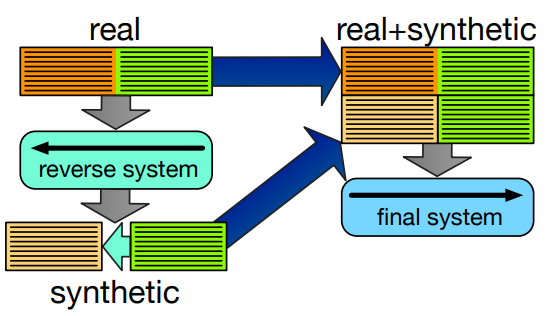
\includegraphics[width=0.55\textwidth]{media/literature/data_argumentation/da_back_trans.png}
\caption[Back-translation synthetic parallel corpus creation]{Back-translation synthetic parallel corpus creation (\cite{hoang_iterative_2018})}
\label{fig:back_trans}
\end{figure}
Research by \cite{sennrich_improving_2016} incorporates monolingual data into \acrshort{NMT} by studying the effect of using back-translation on monolingual data in order to improve translation models.  Without any alterations to the underlying architecture, their findings indicate that adding the synthetic data to the training corpus significantly improved translation quality by $3.4$ BLEU score in both high-resource and low-resource training data sets.


\subsection{Sentence Segmentation}

Sentence segmentation is the process of using punctuation marks within a sentence as delimiters to divide the sentence into multiple partial sentences. When applied to an existing parallel corpus that contains long sentences with punctuation, sentence segmentation can be used as a data augmentation technique. \cite{zhang_corpus_2019} implemented this by generating pseudo-parallel sentence pairs using sentence segmentation with back-translation as follows:
\begin{itemize}
    \item Divide the sentences into a parallel training data set into partial sentences
    \item Back-translate the partial sentences from the target language
    \item Use back-translated data to replace partial sentences from the source language
\end{itemize}

Results of their sentence segmentation implementation demonstrate that the increase of parallel sentence pairs can lead to improvements over baseline \acrshort{NMT} translation performance. In addition, their proposed method outperformed models using the back-translation augmentation method for the Japanese - Chinese 'ASPEC-JC' (\cite{NAKAZAWA16.621}) training corpus.

\subsection{Easy Data Augmentation}
\acrfull{EDA} is a data augmentation technique which aims to improve \acrshort{NLP} text classification performance by creating augmented training data to artificially increase the size of the corpus. It is a corpus augmentation technique that uses a combination of word replacements, insertions, swaps, and deletions. Additional parameters such as the number of augmented sentences per original sentence, and the percentage of words from the original sentence to change allow for fine-tuning of the output relevant to the usage context. For individual sentences in the training data, an augmented sentence is generated using an operation selected randomly from four different techniques:
\begin{itemize}
    \item \textbf{Synonym Replacement:} Select $n$ words at random and replace each one with a synonym
    \item \textbf{Random Insertion:} Insert the synonym of any word into any position. Repeat $n$ times
    \item \textbf{Random Swap:} Swap the position of any two words. Repeat $n$ times
    \item \textbf{Random Deletion:} Randomly delete each word with probability $p$
\end{itemize}

\cite{wei_eda:_2019} found that \acrshort{EDA} increased performance for both recurrent and convolutional neural networks and improvements are most significant when the data was restricted to simulate a low-resource scenario. The additional training data generated and noise from the variety of swaps contribute towards reduced overfitting. In a text classification task, \acrshort{EDA} can achieve the same level of accuracy as the baseline performance of the entire training corpus despite only using only $50$\% of the training corpus. However, \acrshort{EDA} experiments have focussed exclusively on its application to text classification. Although it may be useful for generating additional monolingual data, \acrshort{EDA} cannot be applied to a parallel data set consisting of two different languages due to the replacement that occurs without the use of a language model.

\subsection{Contextual Data Augmentation}

Contextual data augmentation is a type of data augmentation where words are replaced at random using predictions from a language model, based on the context of the word within the sentence. As with other augmentation techniques, the primary aim is to reduce overfitting and improve generalisation of the models that train on the augmented data. 

Although capable of retaining contextual information, contextual data augmentation research is primarily focussed on text classification tasks rather than \acrshort{NMT}. Research by \cite{wu_conditional_2018} and \cite{kobayashi_contextual_2018} are good examples of this, where the augmented data can be fairly similar to the original data making it significantly less beneficial for \acrshort{NMT} training despite remaining useful in \acrshort{NLP} classifiers. This is difficult to overcome due to limitations in the usage of vocabulary without repeating the augmentation process many times for each sentence while maintaining grammatically correct output.
\acrfull{SCDA} is a method of data augmentation proposed by \cite{zhu_soft_2019}, specifically designed for use in \acrshort{NMT} systems. The \acrshort{SCDA} uses a language model that is trained on the same training corpus as the \acrshort{NMT} model, as shown in Figure \ref{fig:scda}.

\begin{figure}[ht!]
\centering
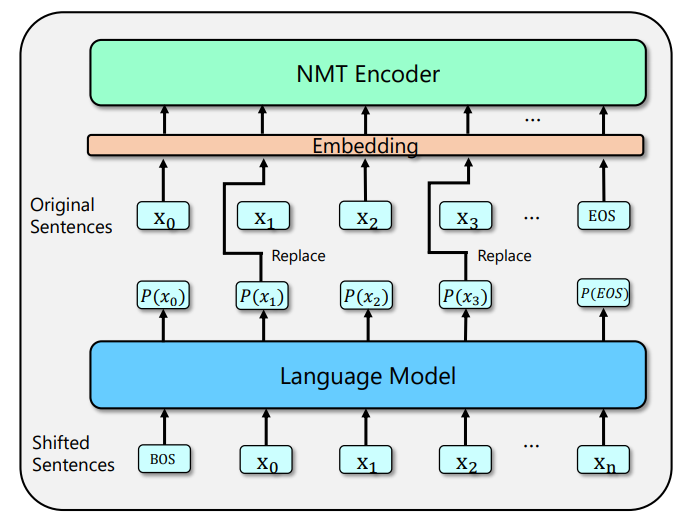
\includegraphics[width=0.58\textwidth]{media/literature/data_argumentation/da_scda.png}
\caption[\acrlong{SCDA} encoder architecture]{\acrlong{SCDA} encoder architecture (\cite{zhu_soft_2019})}
\label{fig:scda}
\end{figure}

The key difference is that random words from the original sentences are replaced with a mix of contextually related words using a probability distribution vector.




Their findings demonstrate that the \acrshort{SCDA} method provides a consistent improvement of more than $1.0$ BLEU score for the transformer model \acrshort{NMT} in comparison to alternative approach baselines using a transformer model with both small and large data sets.


\section{Low-Resource Machine Translation}
\label{sec:2-low_resource_approaches}
This section will explain how using the knowledge gained on a previous task can be achieved through transfer learning and meta learning techniques, improving the performance on a related task where training on high resource languages forms the basis of the initialisation in the neural network of a low-resource language.

\subsection{Existing Scottish Gaelic Machine Translation}
%Existing research on Scottish Gaelic machine translation has focussed on using \acrshort{SMT}

Research by \cite{dowling_leveraging_2019} takes advantage of the increased data availability of a high-resource language (Irish Gaelic) and uses back-translation to create a parallel corpus with Scottish Gaelic, a closely related low-resource language pair. As shown in Figure \ref{fig:lang_pair}, the sentence structure of Irish Gaelic (GA) and Scottish Gaelic (GD) is very similar, making it an ideal choice for back-translation.

\begin{figure}[ht!]
\centering
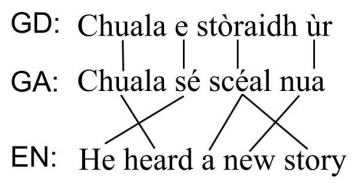
\includegraphics[width=0.4\textwidth]{media/literature/nmt_approaches/lr_gaelic.png}
\caption[Similarities in a closely related language pair]{Similarities in a closely related language pair (\cite{dowling_leveraging_2019})}
\label{fig:lang_pair}
\end{figure}


The \acrshort{SMT} model saw improvements in performance over baseline when combining the synthetic training data with the original training data. The reason stated for not using \acrshort{NMT} in this research was due to the limited corpus size. As \acrshort{NMT} translation quality suffers significantly when models are trained with a low quantity of data, and as demonstrated in research by \cite{dowling_smt_2018}, a well-tailored \acrshort{SMT} model achieves much better translation quality in comparison to an "out-of-the-box" \acrshort{NMT} model for Irish translation. Therefore, the research of low-resource neural machine translation for Scottish Gaelic may contribute towards solving this problem. This project aims to expand upon the existing research and explore the application of \acrshort{NMT} to Scottish Gaelic through the implementation of transfer learning techniques.

\subsection{Transfer Learning}
\label{sec:2-transfer_learning}
As outlined by \cite{torrey_transfer_2009}, transfer learning uses the knowledge gained from a previous task in order to improve model performance in a related task. This concept is illustrated in Figure \ref{fig:transfer}, where knowledge gained from the source domain $A$ is used to help inform the target domain $B$.

\begin{figure}[ht!]
\centering
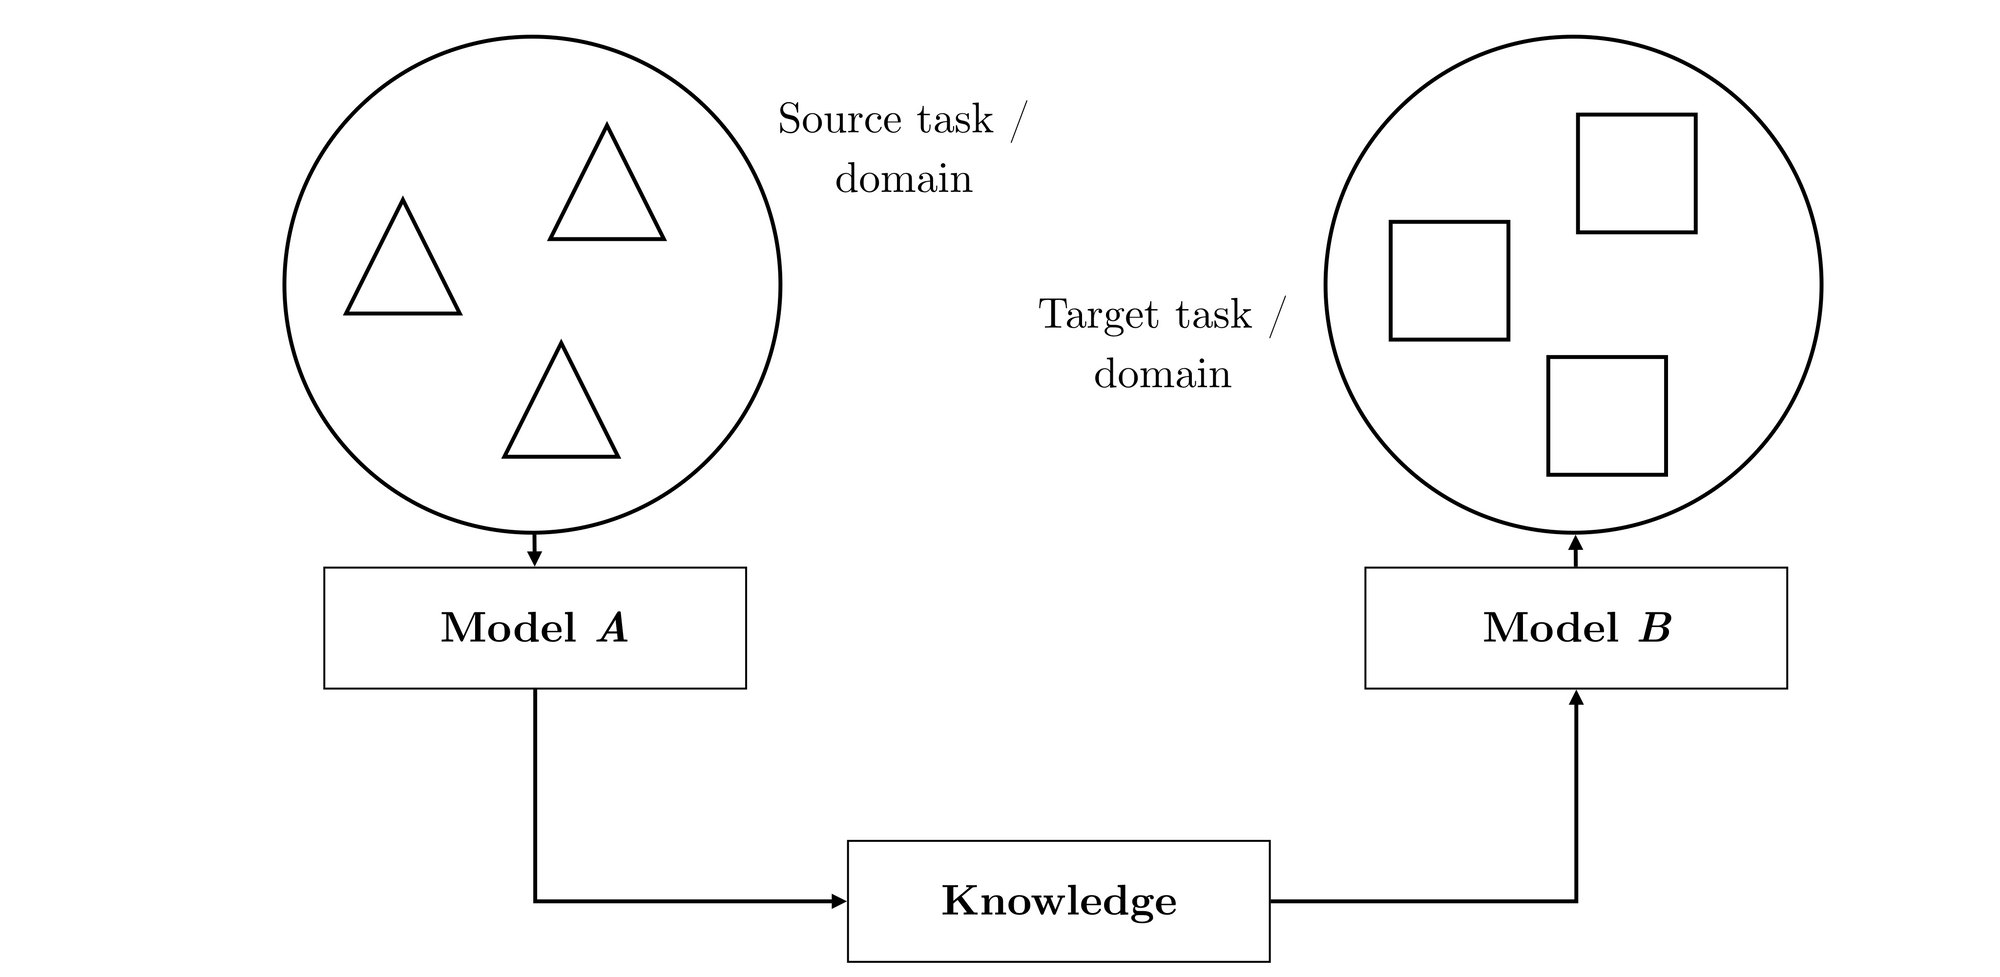
\includegraphics[width=0.8\textwidth]{media/literature/nmt_approaches/transfer.png}
\caption[The process of transfer learning]{The process of transfer learning (\cite{ruder_transfer_2019})}
\label{fig:transfer}
\end{figure}


In a neural machine translation context, this involves training a model with data from a high-resource language and then using that model to initialise the weights of the model that will be trained on the low-resource language.
This was demonstrated in research by \cite{zoph_transfer_2016}, where transfer learning improved the performance of \acrshort{NMT} models for low-resource languages by an average of $5.6$ \acrshort{BLEU} on four different language pairs. Results also suggest that selecting a high-resource language closely related to the low-resource language can improve transfer learning models and therefore translation quality.

However, this contradicts more recent research by \cite{kocmi_trivial_2018} which looks at "trivial transfer learning". Existing transfer learning methods require a degree of language relatedness, whereas trivial transfer learning prioritises data quantity for the high-resource language. Their findings indicate that the relatedness of the language pair is of less importance than the quantity of data used in the initial high-resource language training. Despite being unable to pinpoint the exact reasoning behind the improvement in results, they state that "our observations indicate that the key factor is the size of the parent corpus rather than e.g. vocabulary overlaps".
It is worth noting that \cite{kocmi_trivial_2018} use a transformer neural network instead of the recurrent neural network used by \cite{zoph_transfer_2016}. Research by \cite{popel_training_2018} found that using the transformer model leads to better translation quality, likely contributing towards the contradictory results.


Hierarchical transfer learning seeks to ensure the closeness of the related language pair, as identified in most transfer learning research, while simultaneously addressing the importance of the high-resource data quantity outlined in trivial transfer learning. \cite{luo_hierarchical_2019} achieve this by implementing three distinct stages of training:

\begin{itemize}
  \item Train the model using an unrelated high-resource language pair
  \item Initialise the next model and train on an intermediate language pair
  \item Initialise the final model and train using the low-resource language pair
\end{itemize}

Results indicate improvements of up to $0.58$ \acrshort{BLEU} score in comparison to the aforementioned transfer learning methods that are limited to a parent-child architecture.

\subsection{Meta Learning}
\label{sec-2:meta_learning}

% what is meta learning
Meta learning can be thought of as the machine learning process of "learning how to learn". Observing the performance of different approaches on a variety of tasks and then using this experience to influence the learning process of new tasks to considerably increase the rate of learning (\cite{vanschoren_meta-learning:_2018}).
% talk about model agnostic meta learning
\acrfull{MAML} is a meta learning algorithm proposed by \cite{finn_model-agnostic_2017}, where models are trained to adapt quickly. This leads to good generalisation performance on a new task despite a low quantity of training data.
A diagram of the \acrshort{MAML} algorithm can be seen in Figure \ref{fig:MAML}.

\begin{figure}[ht!]
\centering
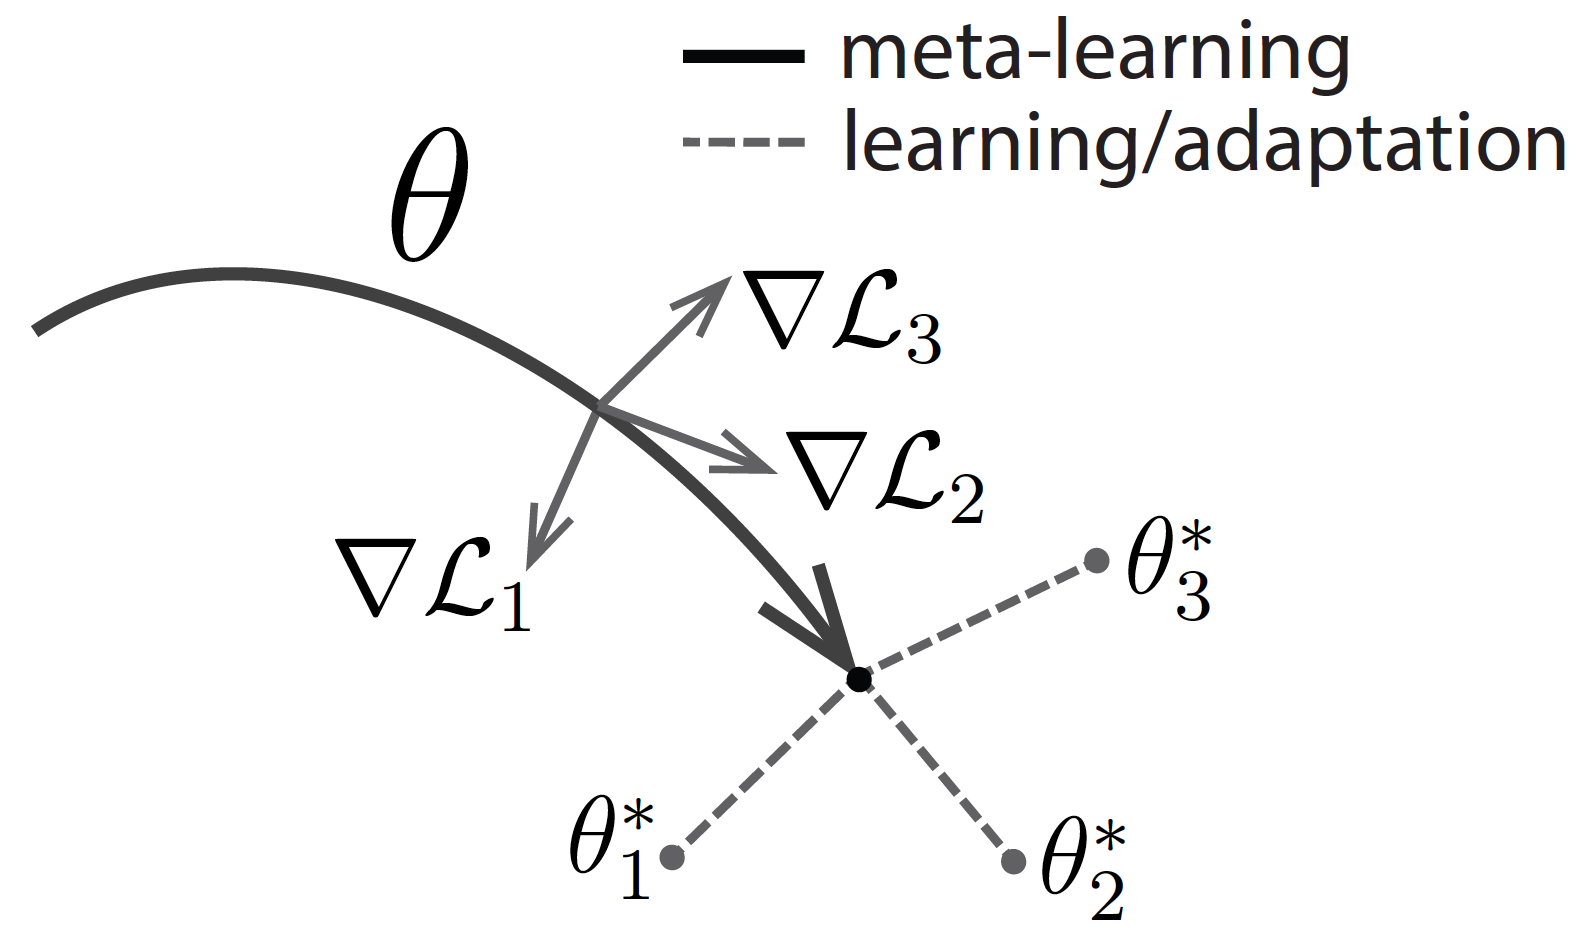
\includegraphics[width=0.40\textwidth]{media/literature/nmt_approaches/maml.png}
\caption[\gls{MAML} algorithm]{An illustration of the \Gls{MAML} algorithm (\cite{finn_model-agnostic_2017})}
\label{fig:MAML}
\end{figure}

Despite the primary focus of \acrshort{MAML} research relating to object recognition, it can be applied to a variety of machine learning problems with any number of training steps or training data because the algorithm still produces a weight initialisation, meaning no additional learning parameters are required.


Research by \cite{gu_meta-learning_2018} is the first of its kind to use \acrshort{MAML} for \acrshort{NMT}. In comparison to the transfer based approach by \cite{zoph_transfer_2016}, results showed further improvements with a BLEU score of $22.04$, despite training data for the low-resource language limited to $16,000$ words (around $600$ parallel sentences). As the corpus size of the low-resource language decreases, transfer learning approaches suffer significantly more than meta learning, which proves the effectiveness of \acrshort{MAML} for low-resource languages. However, as the corpus size increases, the differences in BLEU score between the two approaches are much less significant.

\section{Conclusions}

This chapter reviewed the literature surrounding neural networks and machine translation, leading to approaches for low-resource neural machine translation. 

From the research covered in this review, it is clear that there have been many important developments in machine translation since its origin. Advancements in statistical machine translation and more recently the shift towards neural machine translation with convolutional neural networks and recurrent neural networks have led to significant improvements in translation quality.

As confirmed by the literature, various low-resource \acrshort{NMT} techniques have shown to achieve significantly higher translation quality scores than baseline \acrshort{NMT} approaches on the same low-resource data corpus. Transfer learning has been the main focus of low-resource neural machine translation research, however, new research on meta learning has shown promising results with improvements over transfer learning. A variety of automatic evaluation metrics that can be used for evaluating the performance of translation models were identified in the research. \acrshort{BLEU} score will be the most beneficial metric to use during training and evaluation due to its high correlation to human translators and widespread adoption among virtually all other machine translation research.

Limitations of recent research primarily involve the scope of each implementation. There are many techniques and implementation decisions that have shown to improve translation quality, however, the majority of the research goes into great detail about one particular choice. Understandably, individual papers have a clear focus, but there is an identifiable gap in the research regarding the impact of using a combination of the aforementioned techniques. Data augmentation techniques such as back-translation have shown to improve \acrshort{NMT} quality on baseline \acrshort{NMT} approaches, so it is worth investigating what the impact when used with low-resource \acrshort{NMT} approaches. There is also no existing research for Scottish Gaelic \acrshort{NMT} systems as prior research was limited to statistical machine translation due to the large quantity of training data required with generic \acrshort{NMT} approaches. Transfer learning has shown promising results in other low-resource languages, so it may be a good alternative for Scottish Gaelic.

Based on the review of literature, the low-resource \acrshort{NMT} techniques that the project implements are trivial transfer learning and hierarchical transfer learning. The initialisation of a neural network with the weights of a previously trained neural network in a similar domain helps to aid the translation quality, particularly in a low-resource context. Experimentation in regards to the relatedness of the language pair, particularly Irish Gaelic which also has a very similar sentence structure, will identify whether either the quantity or relatedness of data is of higher importance for Scottish Gaelic.
